\documentclass{beamer}

\usepackage[portuguese]{babel}
\usepackage[utf8x]{inputenc}
\usepackage{default}
\usetheme{PaloAlto}
\usecolortheme{seahorse}

\title{Projeto Pindí}
\author{José A. Neto, José P. Neto, Lucas A. Moura, \\
        Marcos S. Ramos, Maria Eugênia Santos,\\
        Matheus F. Pimenta, Pablo A. Urbizagastegui,\\
        Rodrigo S. Melo, Thaynara R. Santana, \\
        Tuane T. Fonseca, Vanessa O. Ribeiro}

\date{\today}

\institute{\textbf{Universidade de Brasília - Faculdade do Gama}} 

\begin{document}

%SLIDE INICIAL DE APRESENTAÇÃO 3 min
\begin{frame}
  \titlepage
\end{frame}
  
%SLIDES == INTRODUÇÃO
\section{Introdução}
\begin{frame}
  \frametitle{Tarefas do dia a dia...}
  \begin{center}
    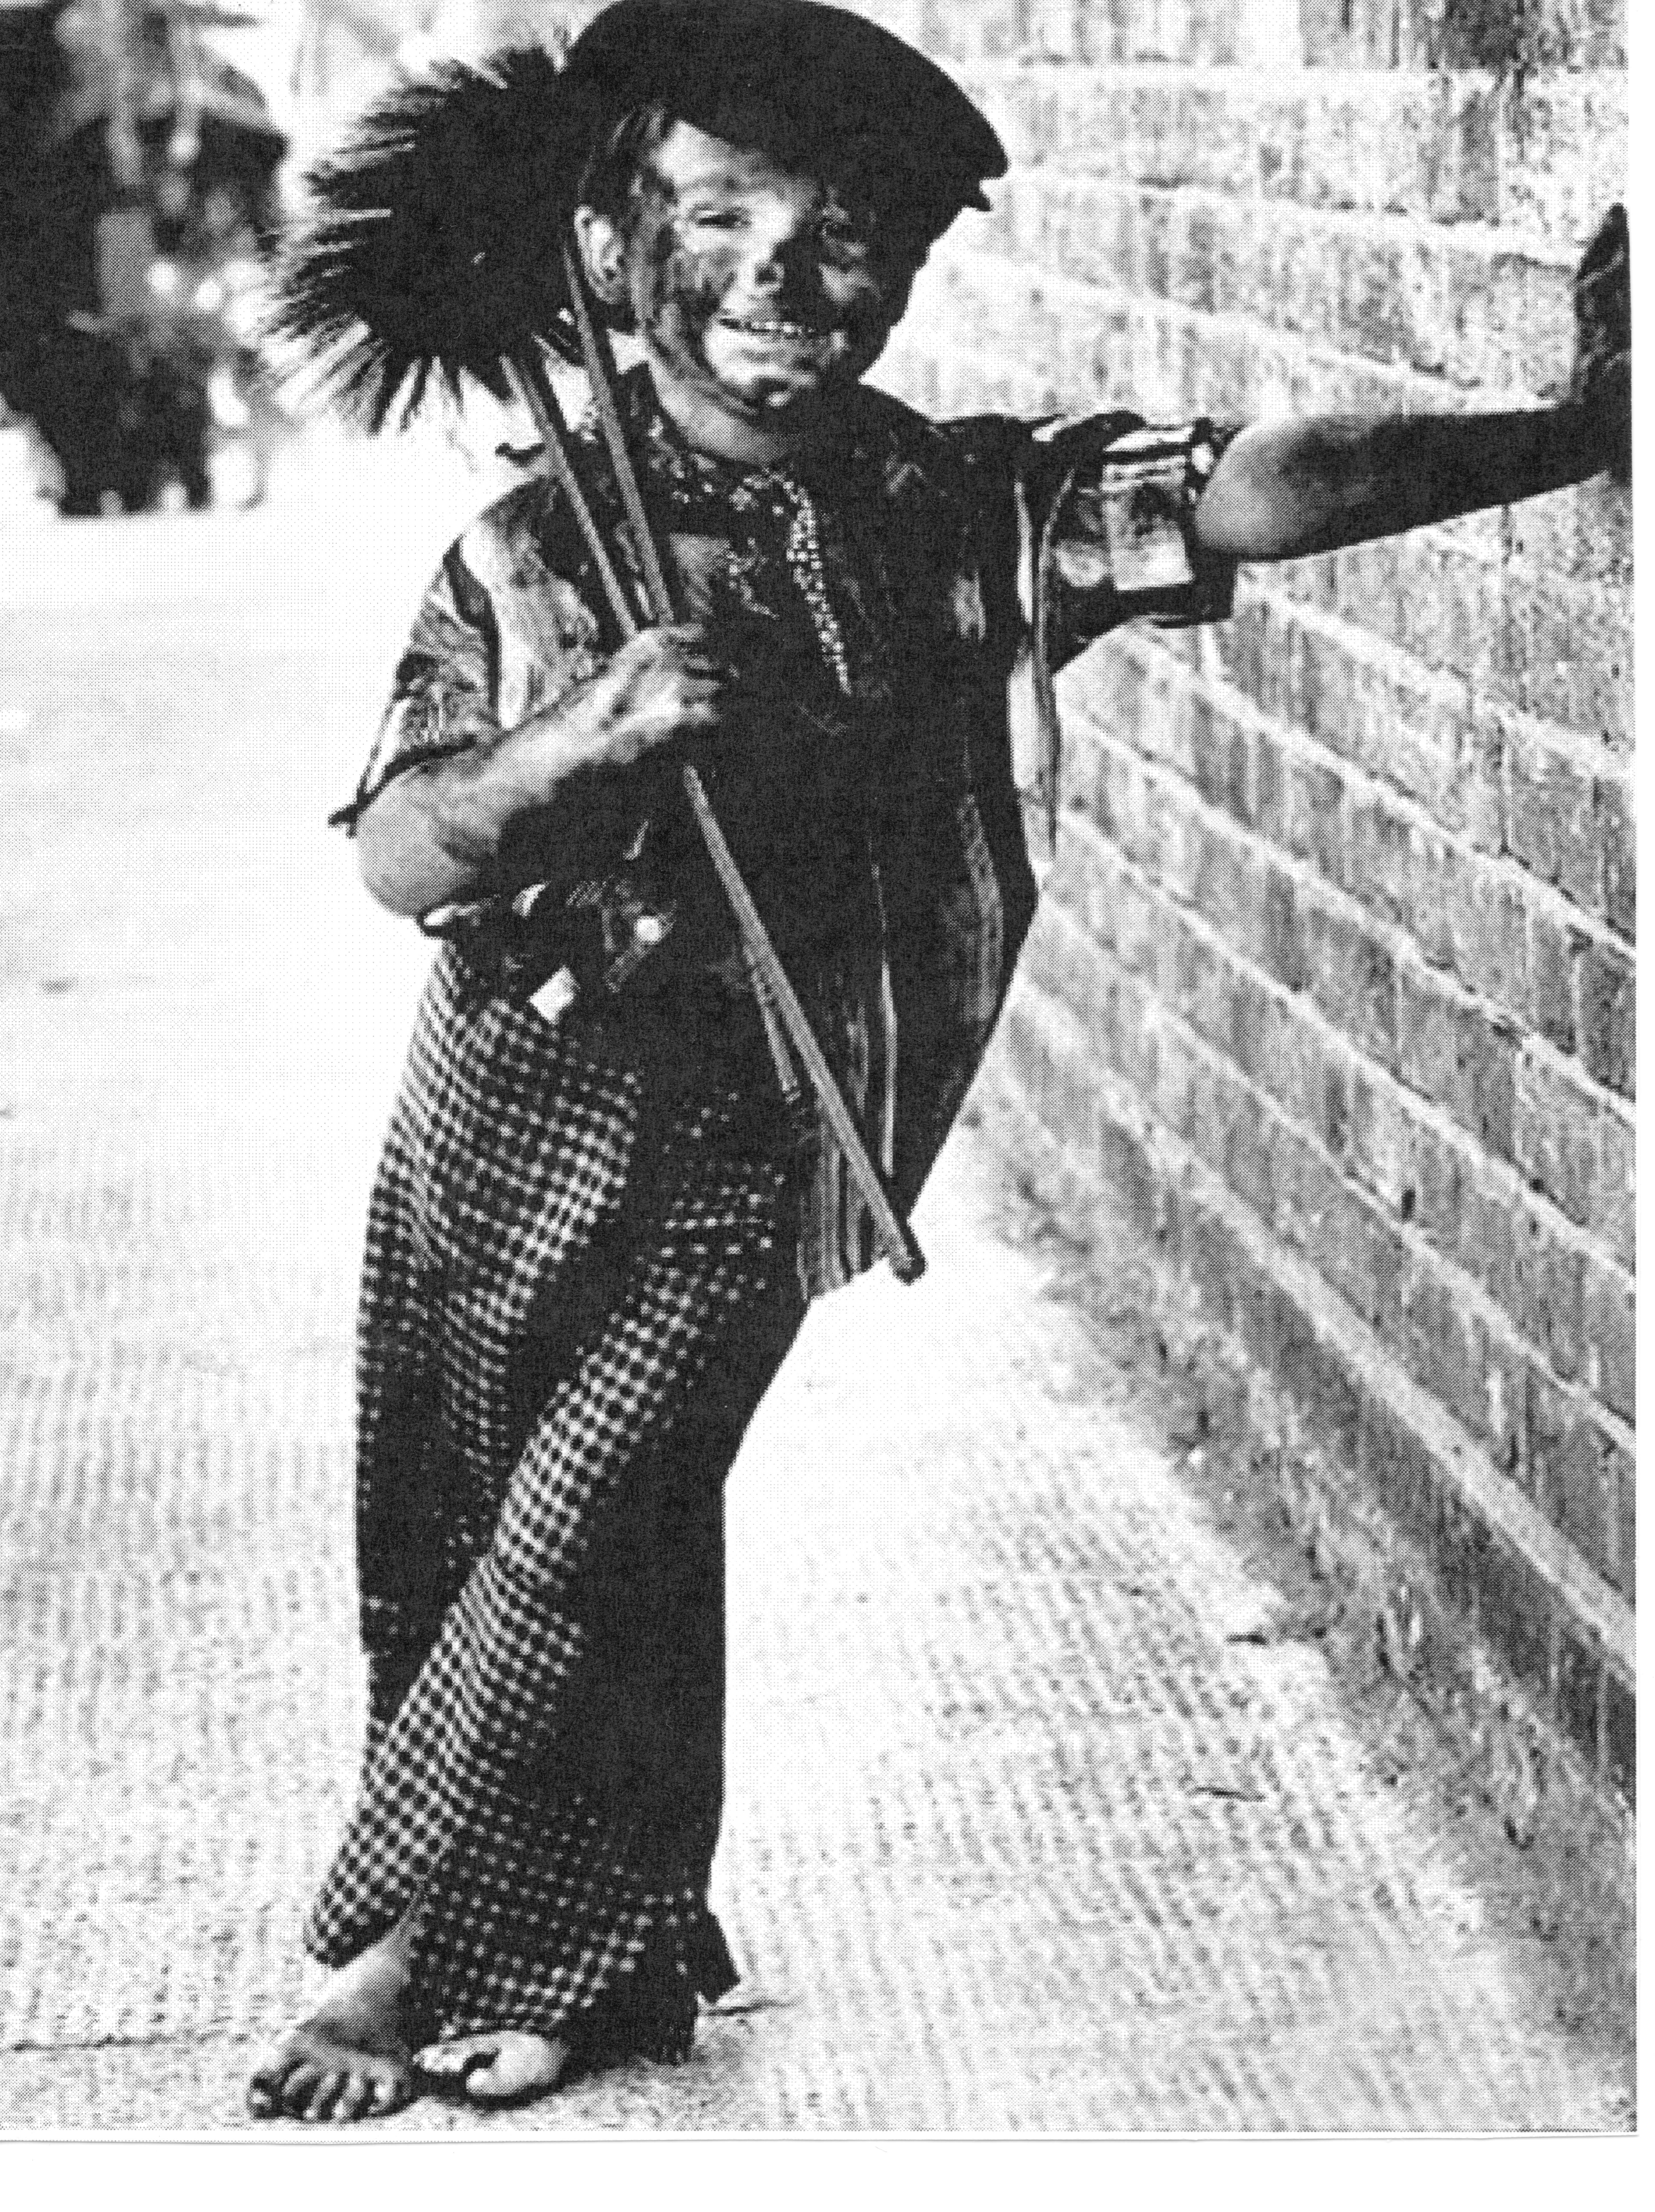
\includegraphics[height = 3in, width = 2in]{images/sweep.jpg}
  \end{center}
\end{frame}

\begin{frame}
  \frametitle{Estresse diário}
  \begin{center}
    \includegraphics[height = 2in, width = 3in]{images/rage.jpeg}
  \end{center}
\end{frame}

\begin{frame}
  \frametitle{Mudança da sociedade}
  \begin{center}
    \includegraphics[height = 1.5in, width = 2in]{images/sozinho.jpg}
  \end{center}
\end{frame}

\begin{frame}
 \frametitle{Valores}
 \begin{center}
    \includegraphics[height = 2in, width = 3in]{images/market.png}
  \end{center}
\end{frame}

%SLIDES == Top Down - 2 min
\section{Visão do produto}
\begin{frame}
	Produtos Existentes	
\end{frame}

\begin{frame}
  \frametitle{Produtos existentes}
  \begin{figure}[ht]
  \includegraphics[width=.4\textwidth]{images/dyson_360.jpg}
  \caption{Dyson 360 Eye}
  \end{figure}
  \begin{itemize}
  	\item Sistema de limpeza extremamente eficiente
  	\item Mapeamento do terreno por processamento de imagens
  	\item US\$ 1.000,00 (ainda não disponível)
  \end{itemize}
\end{frame}

\begin{frame}
  \frametitle{Produtos existentes}
  \begin{figure}[ht]
  \includegraphics[width=.4\textwidth]{images/irobot.jpg}
  \caption{Roomba iRobot}
  \end{figure}
  \begin{itemize}
  	\item Sistema de limpeza razoável
  	\item Mapeamento do terreno por sensores
  	\item US\$ 479,00 (R\$3.000,00)
  \end{itemize}
\end{frame}

\begin{frame}
  \frametitle{Produtos existentes}
  \begin{figure}[ht]
    \includegraphics[width=.30\textwidth]{images/deebot.jpg}
    \caption{Ecovacs Deebot}
  \end{figure}
  \begin{itemize}
  	\item Sistema de limpeza razoável
  	\item Movimentação aleatória (desliga quando acaba a bateria)
  	\item R\$599,00
  \end{itemize}

\end{frame}

\begin{frame}
  \frametitle{Nicho escolhido}
  \textbf{Desafio:} desenvolver um produto voltado para o mercado nacional, na mesma faixa de preço do Deebot porém com mais recursos.
\end{frame}

%SLIDES == EXEMPLO DIAGRAMA DE ESTADOS
\section{Apresentação do produto}
\begin{frame}
  %TODO
  \frametitle{Escopo}
  \begin{itemize}
  	\item Obstáculos "grandes" (cadeiras, sofás, mesas etc.)
  	\item Poeira seca
  	\item Piso de cerâmica ou similar
  	\item Sem carpete ou tapete
  \end{itemize}
  
  %TODO colocar do lado da lista
  \begin{figure}
    \includegraphics[width=.30\textwidth]{images/sala.jpg}
  \end{figure}
  
\end{frame}

\begin{frame}
  %TODO
  \frametitle{Caracterização}
  \begin{itemize}
  	\item Movimentação autônonoma
  	\item Varrição
  	\item Aspiração
  \end{itemize}
\end{frame}

\begin{frame}
  %TODO
  \frametitle{Limitações}
  \begin{itemize}
  	\item Não substitui uma limpeza completa: apenas a complementa
  	\item ??
  	\item ??
  \end{itemize}
\end{frame}

\section{Viabilidade}
\begin{frame}
  \frametitle{O que foi feito}
  \textbf{Objetivo:} Validar a capacidade do grupo e validar a efetividade da solução escolhida.
\end{frame}

\begin{frame}
  \frametitle{O que foi feito}
  Cada elemento chave do projeto foi testado individualmente. São eles:
  \begin{itemize}
  	\item Sistema de limpeza por varrição
  	\item Sistema de limpeza por aspiração
  	\item Movimentação e desvio de obstáculos
  \end{itemize}
  Para cada elemento foi criado um protótipo.
\end{frame}

\begin{frame}
  \frametitle{O que foi feito}
  \textbf{Objetivo:} Aprimorar os protótipos desenvolvidos e integrar todos os sistemas em um único conjunto.
\end{frame}

\begin{frame}
  \frametitle{O que vamos fazer}
  \begin{itemize}
  	\item Melhorias no algoritmo de movimentação
  	\item Integração dos sistemas de limpeza
  	\item Controle de tração e direção otimizados
  	\item Sistema de alimentação mais robusto
  \end{itemize}
\end{frame}

\section{Fim}
\begin{frame}
	\frametitle{Fim}
	Obrigado!
\end{frame}

\end{document}
